\chapter{Trough Filling and Primitive Network Completion}

In this chapter we demonstrate how to bolster some of the primitive segmentation methods using extended ideas of Frangi filters. Solve the network completion problem using a strict Frangi filtering and basic morphological arguments.

First, we introduce the concept of the signed Frangi filter. As shown in two examples in \cref{fig:signsweep-1} and \cref{fig:signsweep-2}, we can simulataneously calculate for a dark background and a light background. Since the Frangi filter normally throws away any response where $\lambda_2 < 0$ (if dark curvilinear features are desired) or $\lambda_2 >0$ (if light curvilinear features are desired), we lose no computation time at all. After computing the multiscale result, we can easily separate these into a positive and a negative strain, which we will denote
$\Vmax^{(+)}$ and $\Vmax^{(-)}$. Our $\Vmax^{(+)}$ is the same as our $\Vmax$ before, and $\Vmax^{(-1)}$ is the same result as if we had taken the Frangi filter while only looking for the opposite type (light/dark) curvilinear feature. Plotting $\Vmax$ over a scale of $[-1,1]$ demonstrates an interesting effect. Whereas the Frangi filter generally is not reliable in terms of accurately predicting widths, we \textit{can} get a sense of the width by looking at where there is a relatively strong response of opposite sign.

\begin{figure}[p] \centering
	\subfloat{		\label{fig:signsweep-1p}\includegraphics[width=\linewidth]{{{signsweep_stitch_BN2315363_plate}}}
	} \\[-0.5cm]
	\subfloat{		\label{fig:signsweep-1i}\includegraphics[width=\linewidth]{{{signsweep_stitch_BN2315363_inset}}}
	} \\[-0.5cm]
	\subfloat{		
		\label{fig:signsweep-1c}\includegraphics[width=.75\linewidth]{{{signsweep_colorbar}}}
	} \\
	
	\caption{Signed Frangi output (plate and inset) (Example 1)}
	\label{fig:signsweep-1}
\end{figure}

\begin{figure}[p] \centering
	\subfloat{		\label{fig:signsweep-2p}\includegraphics[width=\linewidth]{{{signsweep_stitch_BN5280796_plate}}}
	} \\[-0.5cm]
	\subfloat{		\label{fig:signsweep-2i}\includegraphics[width=\linewidth]{{{signsweep_stitch_BN5280796_inset}}}
	} \\[-0.5cm]
	\subfloat{		
		\label{fig:signsweep-2c}\includegraphics[width=.75\linewidth]{{{signsweep_colorbar}}}
	} \\
	% should i use the real sample names? or obfuscate?
	\caption{Signed Frangi output (plate and inset) (Example 1)}
	\label{fig:signsweep-2}
\end{figure}

That is, at the "foot" of every trough on either side, we can see a bordering curvilinear structure of opposite sign. We perform strict Frangi filtering and separate the positive and negative components. We then perform a different threshold as each--a strict one (say $\alpha^{(+)} > .4$) for the conventional $\Vmax$, and a much looser one for our opposite signed $\Vmax^{(-)} > \alpha^{(-)} = .05.$. We also truncate the scales we consider for calculating $\Vmax^{-}$, say only the first 12 of 20.

We then perform a thinning operation on our positive Frangi response. We will refer to this thinned approximation as the ``spine'' and the (un-thinned) opposite signed component as the ``margin.'' For each pixel on the thinned spine, we iterate over disks of integer radius and dilate the pixel by a disk of that radius if that disk coincides with a margin point. 

\section{Primitive Network Completion}

One of the biggest shortcomings of our demonstrated segmentation methods is that they frequently result in gaps in parts of the network. We demonstrate a way to rectify this problem in certain situations, and then discuss how to extend these arguments to fill larger, more uncertain gaps.

First, once we've produced a segmentation, we thin it down with \cite{thinning} and look for endpoints of an otherwise connected point. Using a $3\times 3$ structuring element, we iterate over each pixel and identify how many local neighbors it has. If a pixel has zero or one local neigbors, we identify it as an endpoint of the partial network. After identifying these endpoints, we assign each a label $(i,j)$ depending on where the neighboring pixel is located, as according to \cref{fig:endpoint_labels}. We deem two endpoints potentially connectible only if they're not connected on the same side. That is, their labels $(i,j)$ and $(i',j')$ must have $i\ne i'$ or $j\ne j'$ (unless $i$ or $j$ is 1). For example, if an endpoint is connected to the partial network on its top side, any endpoint that connects to it cannot also be connected to a network on its top. If a pixel has no connections at all, with label $(1,1)$, we do not restrict its connetions at all. To save time (though we don't anticipate it will affect the result much), we also restrict pais from being more than a set distance away (in this case, 100 pixels in Euclidean length).

\begin{figure}
	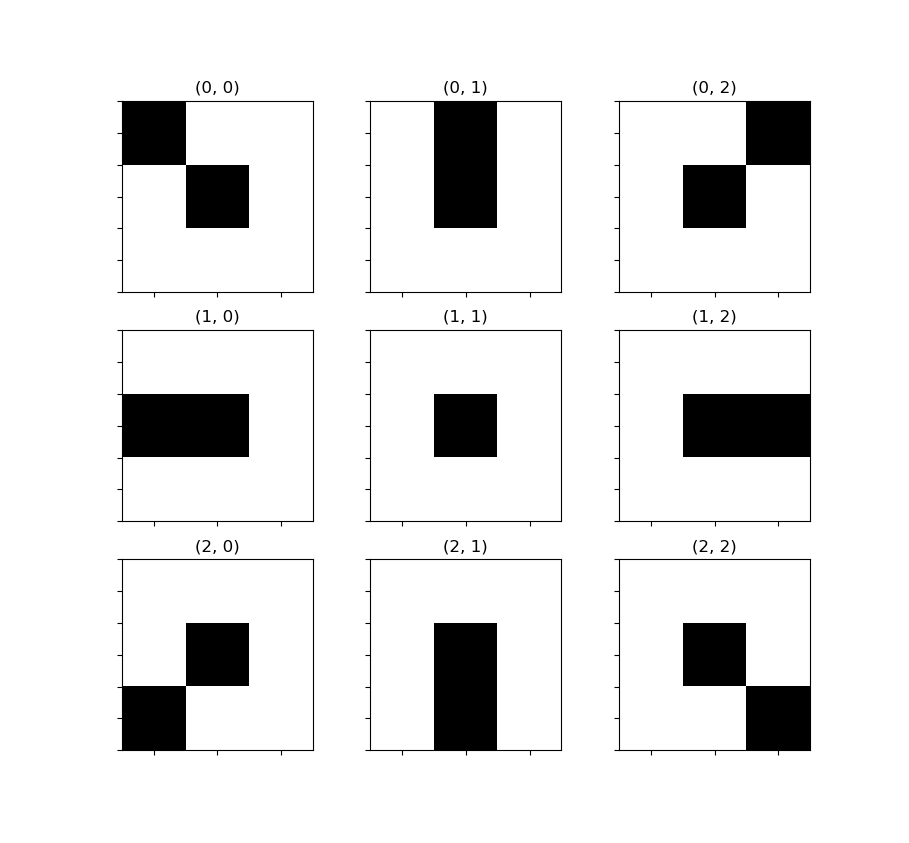
\includegraphics[width=.85\textwidth]{endpoint_labels}
	\caption{Endpoints labels based on adjacent neighbor location}
	\label{fig:endpoint_labels}
\end{figure}

After we limit the connections, we consider each pair of endpoints and draw a straight line segment between the two. If that passes through a point where $\Vmax$ is 0, we disallow that pair as well. We also disallow any line which crosses any part of the network which is known to exist.
Finally, from the list of all remaining pairs of endpoints, we simply select the path along which the maximum mean value of $\Vmax$ is achieved. \cref{fig:network-completion-all-pairs} shows non-violating paths between end-point pairs, and \cref{fig:network-completion} shows a partially completed network (in yellow) overlaid on $\Vmax$.



\begin{figure}
	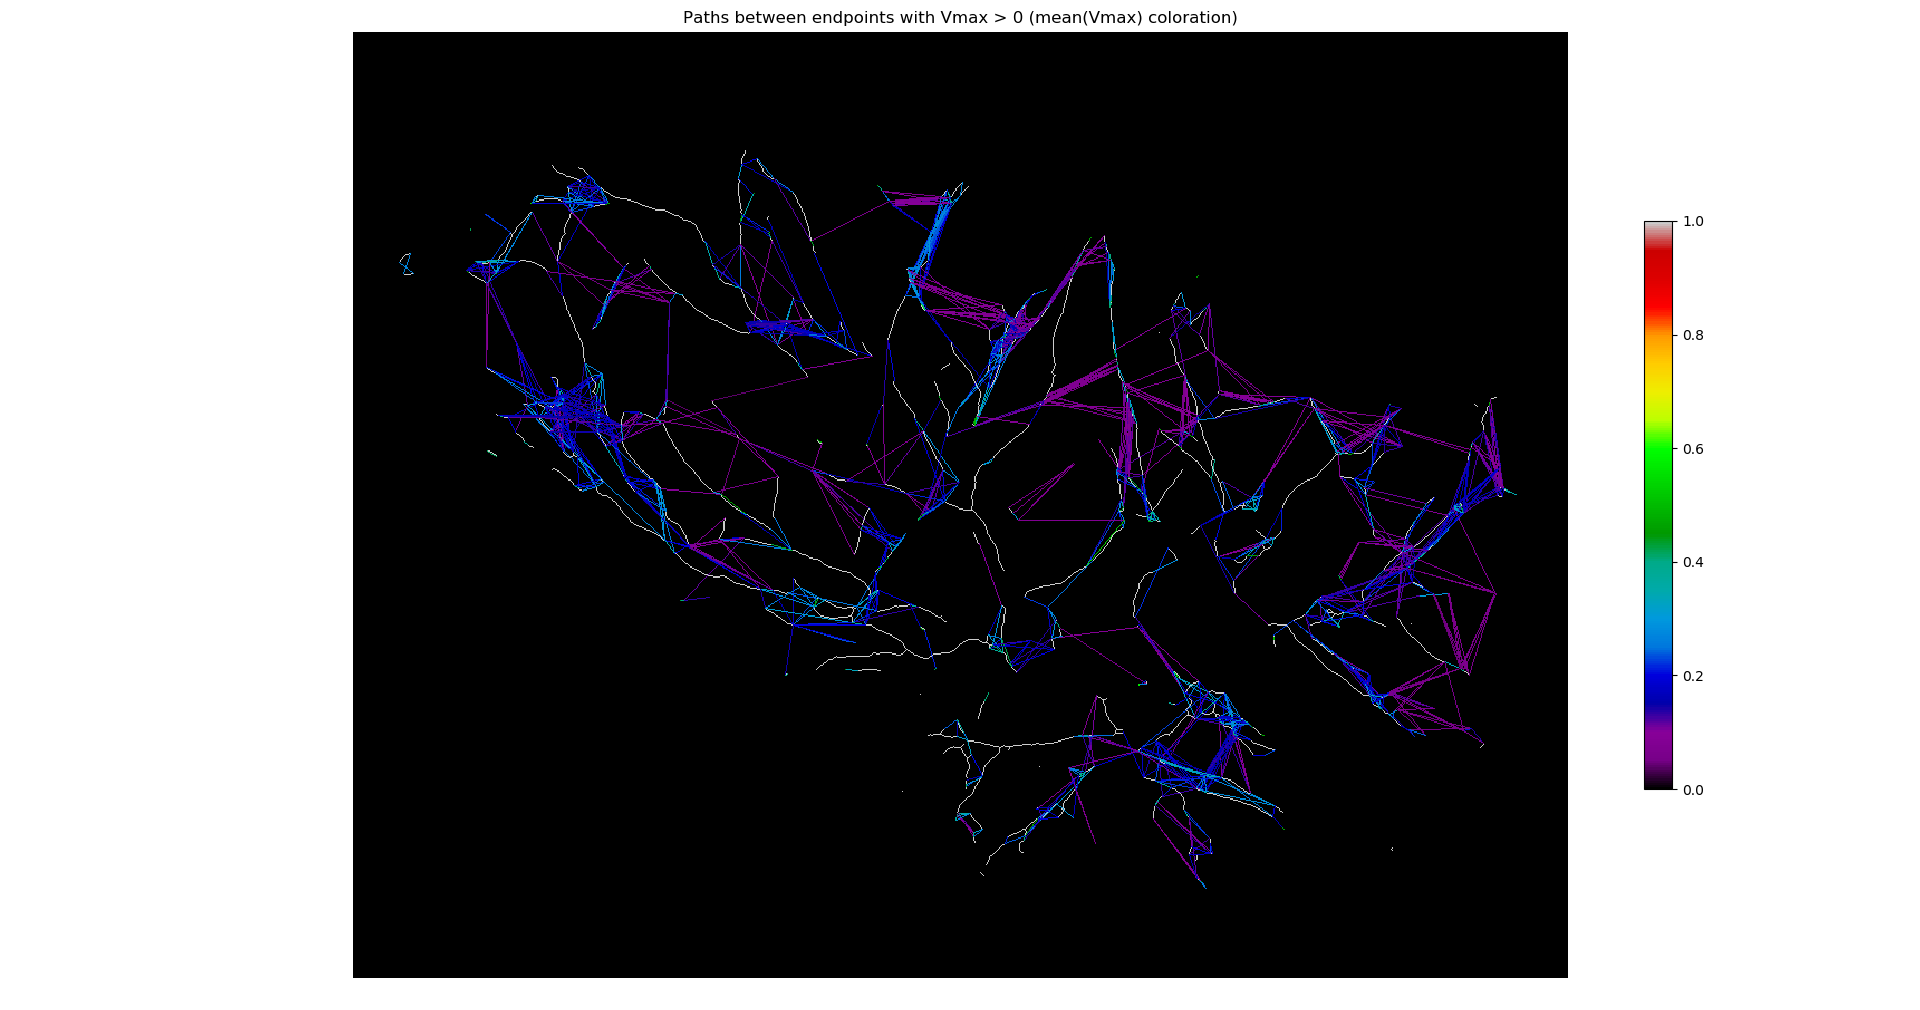
\includegraphics[width=\linewidth]{paths_between_endpoints_positive_score}
	\caption{All lines between endpoints with nonzero $\Vmax$}
	\label{fig:network-completion-all-pairs}
\end{figure}
\begin{figure}
	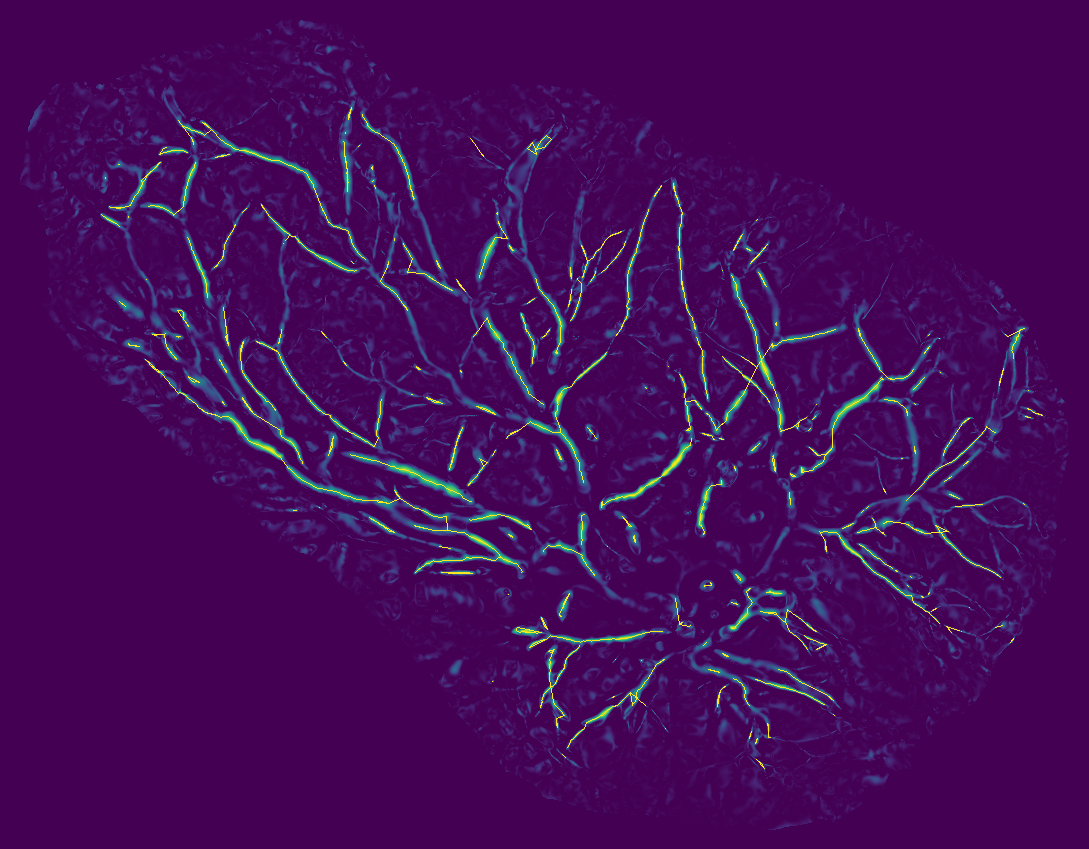
\includegraphics[width=\linewidth]{completed_by_nearest_to_line_mash}
	\caption{Partially completed network}
	\label{fig:network-completion-end-result}
\end{figure}

We show the complete process for comparison on two different samples. 

\begin{figure}
	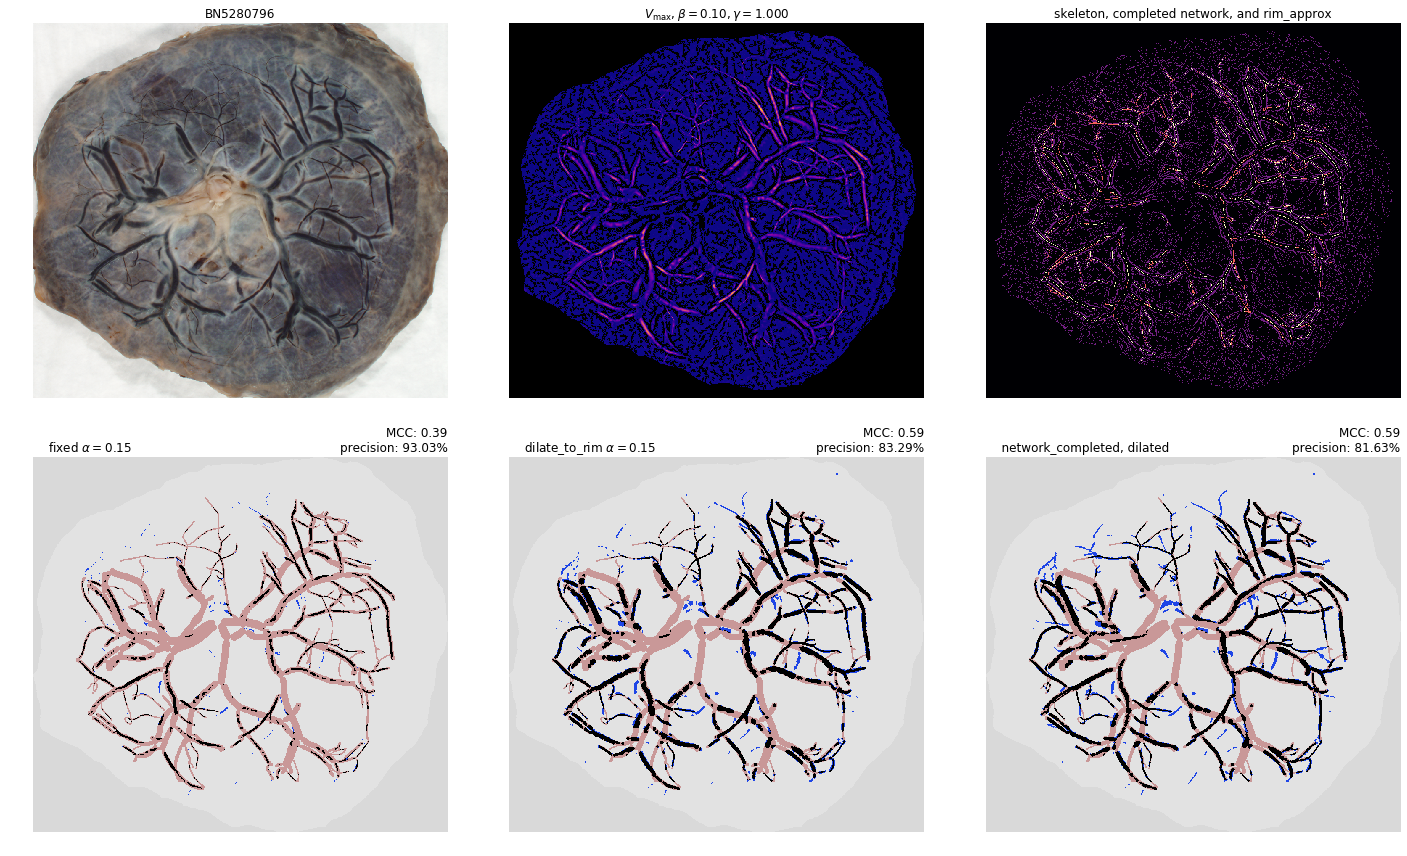
\includegraphics[width=\linewidth]{sample_network_completion}
	\caption{Trough Dilation and Network Completion (Example 1)}
	\label{fig:network-completion-demo-1}
\end{figure}
\begin{figure}
	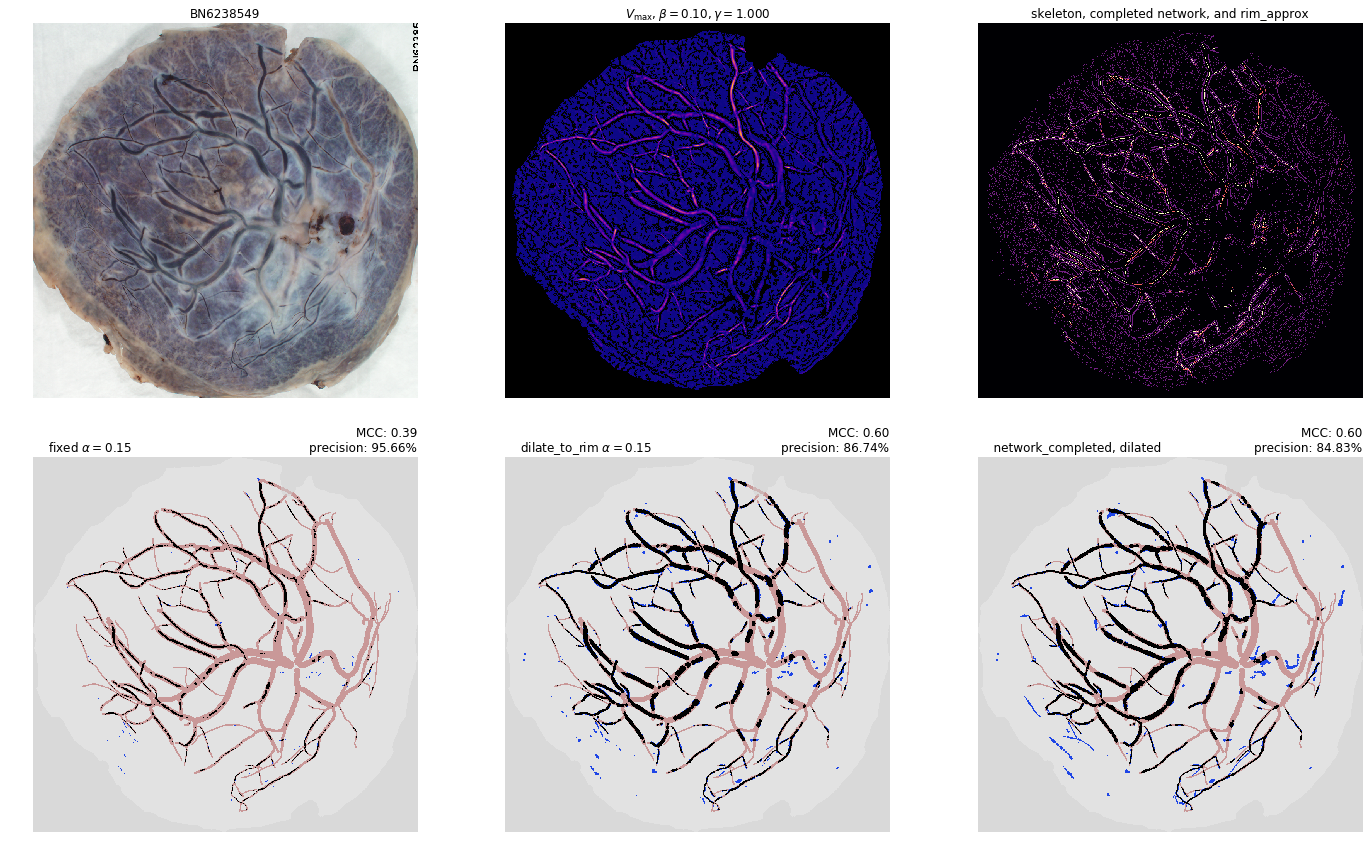
\includegraphics[width=\linewidth]{sample_network_completion_2}
	\caption{Trough Dilation and Network Completion (Example 2)}
	\label{fig:network-completion-demo-2}
\end{figure}


